\documentclass[a4paper]{ltjsarticle}

\usepackage[dvipdfmx]{graphicx}
\usepackage[dvipdfmx,hidelinks,pdfusetitle]{hyperref}
\hypersetup{
    colorlinks=false,
    bookmarksnumbered=true,
    pdfborder={0 0 0},
    bookmarkstype=toc
}
\usepackage[nobreak]{cite}
\usepackage{pxjahyper}
\usepackage{amsmath}
\usepackage{tikz}

\usetikzlibrary{datavisualization}
\usetikzlibrary{positioning}
\usetikzlibrary{shapes.geometric, shapes.misc}
\usetikzlibrary{patterns}
\usetikzlibrary{calc}

\begin{document}

\begin{itembox}[l]{東京大学 2015年 文科 第2問}
    座標平面上の2点 $A(-1, 1),\ B(1, -1)$ を考える.また, P を座標平面上の点とし,その $x$ 座標の絶対値は1以下であるとする.次の条件 (i) または (ii) を満たす点 P の範囲を図示し,その面積を求めよ.

    \begin{enumerate}[label=(\roman*)]
        \item 頂点の $x$ 座標の絶対値が1以上の2次関数のグラフで,点 A, P, B をすべて通るものがある.
        \item 点 A, P, B は同一直線上にある.
    \end{enumerate}
\end{itembox}

以下,$|x|\leq 1$ において, P の存在範囲 $D$ を考える.

\begin{itemize}
    \item[(i) のとき] 2次関数 $y=ax^2+bx+c$ のグラフが2点 A, B を通るならば,

        \begin{equation}
            y=ax^2-x-a\label{eq:1}
        \end{equation}

        と表せる.\eqref{eq:1} は

        \begin{equation*}
            y=a(x-\frac{1}{2a})^2-a-\frac{1}{4a}
        \end{equation*}

        となるので,頂点の $x$ 座標の条件より,

        \begin{align}
             & \left|\frac{1}{2a}\right|\geq 1\nonumber                                   \\
             & \therefore\quad |a|\leq \frac{1}{2}\quad\text{かつ}\quad a\neq 0\label{eq:2}
        \end{align}

        P の範囲は\eqref{eq:2} のもとで\eqref{eq:1}が通る部分である.

    \item[(ii) のとき] (ii)を満たす点 P は,直線 $y=-x$ 上にあるが,これは\eqref{eq:1}で $a=0$ とおいたものに等しい.
\end{itemize}

以上,(i), (ii) より, $-\frac{1}{2}\leq a\leq\frac{1}{2}$ のもとで,\eqref{eq:1}が通り得る部分が $D$ である.したがって, $|x|\leq 1$ において

\begin{equation}
    \text{「}\eqref{eq:1}\text{を}a\text{の方程式}a(x^2-1)=x+y\text{とみたとき,}-\frac{1}{2}\leq a\leq\frac{1}{2}\text{の範囲に解を持つ」}\label{eq:3}
\end{equation}

条件を求めればいよい.

\begin{enumerate}[label=(\Roman*)]
    \item $x^2=1$ のとき\\

          \eqref{eq:3}より, $x+y=0$\quad つまり\quad $(x, y)=(1,\ -1),\ (-1,\ 1)$

    \item $x^2< 1$ のとき\\

          \begin{equation*}
              a=\frac{x+y}{x^2-1}
          \end{equation*}

          であるから,

          \begin{equation*}
              -\frac{1}{2}\leq\frac{x+y}{x^2-1}\leq\frac{1}{2}
          \end{equation*}

          ここで, $x^2-1<0$ より,これは

          \begin{align}
               & -\frac{1}{2}(x^2-1)\geq x+y\geq\frac{1}{2}(x^2-1)\nonumber                      \\
               & \therefore\quad \frac{1}{2}(x^2-1)-x\leq y\leq-\frac{1}{2}(x^2-1)-x\label{eq:4}
          \end{align}

          と同値.

          \eqref{eq:4}で $x=\pm 1$ とおくと, $y=\mp 1$ (複合同順) となるので,(I), (II) をあわせて, $D$ は $|x|\leq 1$ かつ\eqref{eq:4}であり,図示すると,下図の斜線部分となる(境界を含む).

          \begin{figure}[!ht]
              \centering
              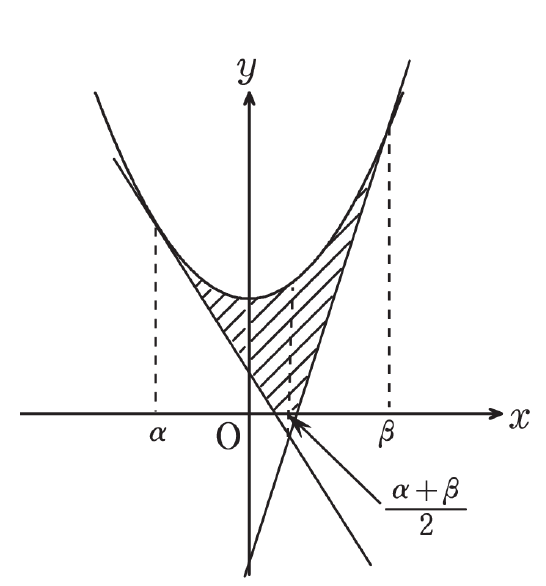
\includegraphics[width=0.5\textwidth]{f1.png}
          \end{figure}

          求める面積は,直線 $y=-x$ に関する対称性により,

          \begin{align*}
               & 2\int_{-1}^{1}\left\{-\frac{1}{2}(x^2-1)-x-(-x)\right\}dx \\
               & =2\int_{-1}^1\left\{-\frac{1}{2}(x^2-1)\right\}dx         \\
               & =2\left[-\frac{1}{6}x^3+\frac{1}{2}x\right]_{-1}^1        \\
               & =\frac{4}{3}
          \end{align*}

          となる.
\end{enumerate}

\end{document}
